% F090｜给定直角边穷举勾股整数数组｜03_proof.tex
% 继承上传模板的 LaTeX 环境；当前条目的内容独立编写。
\clearpage
\begin{proofbox}
\textbf{\textcolor{CProof}{证明一（最低门槛）：勾股定理与平方差}}
\par\medskip
\begin{center}
% F090｜factor 原创简明教学示意图
\begin{tikzpicture}[>=stealth,scale=.92]
\node[draw,rounded corners,fill=teal!10] (a) at (0,0){$a^2=c^2-b^2$};
\node[draw,rounded corners,fill=orange!10] (b) at (5.1,0){$a^2=(c-b)(c+b)$};
\draw[->,thick] (a)--(b);
\node at (2.7,-1){\small 把两平方之差变成两个整数的乘积};
\end{tikzpicture}

\end{center}
\medskip
从 $a^2+b^2=c^2$ 出发，移项得 $a^2=c^2-b^2=(c-b)(c+b)$。等式右边是两个正整数因数，所以它们必是 $a^2$ 的一组因数对。
\end{proofbox}
\clearpage
\begin{proofbox}
\textbf{\textcolor{CProof}{证明二（最快）：从因数对重新构造三边}}
\par\medskip
\begin{center}
% F090｜convert 原创简明教学示意图
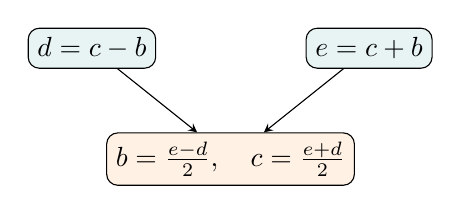
\begin{tikzpicture}[>=stealth,scale=.88]
\node[draw,fill=teal!9,rounded corners] (a) at (0,0){$d=c-b$};
\node[draw,fill=teal!9,rounded corners] (b) at (4,0){$e=c+b$};
\node[draw,fill=orange!10,rounded corners] (c) at (2,-1.6){$b=\frac{e-d}{2},\quad c=\frac{e+d}{2}$};
\draw[->] (a)--(c);\draw[->] (b)--(c);
\end{tikzpicture}

\end{center}
\medskip
取 $0<d<e$，$de=a^2$，且 $d,e$ 同奇同偶。令 $b=(e-d)/2$、$c=(e+d)/2$，可得 $b,c$ 为正整数且\[c^2-b^2=\frac{(e+d)^2-(e-d)^2}{4}=de=a^2.\]所以每个合格因数对都能形成一组。
\end{proofbox}
\clearpage
\begin{proofbox}
\textbf{\textcolor{CProof}{证明三（最完整）：为什么不重不漏}}
\par\medskip
\begin{center}
% F090｜pairs 原创简明教学示意图
\begin{tikzpicture}[>=stealth,scale=.94]
\node[draw,rounded corners,fill=teal!8] (a) at (0,0){$9^2=81$};
\node[draw,rounded corners,fill=orange!8,align=center] (b) at (4.2,0){$1\times81$\\$3\times27$\\$9\times9$};
\node[draw,rounded corners,fill=teal!13,align=center] (c) at (8.5,0){$(9,40,41)$\\$(9,12,15)$\\$b=0$ 排除};
\draw[->,thick] (a)--(b);\draw[->,thick] (b)--(c);
\end{tikzpicture}

\end{center}
\medskip
给定一组正整数解 $(a,b,c)$，因数对必为 $(c-b,c+b)$，无法有第二组不同因数对对应同一个 $(b,c)$。反之，符合条件的因数对又唯一给出 $(b,c)$。于是\textbf{一组解对应一组因数对}，枚举完就找全了。
\end{proofbox}
